\section{Introduction}
\label{sec:intro}

The \ac{LISA} gravitational-wave observatory, planned for launch in the mid-to-late
2030s~\cite{LISA:2017pwj, Colpi:2024xhw}, will unlock our ability to observe the universe
in the low-frequency gravitational-wave band~\cite{LISA:2022yao}.

A key science target
for \ac{LISA} is the observation of \acp{MBHB}. The problem of observing and characterizing
these mergers has been explored over the last two decades, primarily through the LISA Data
Challenges~\cite{Arnaud:2006gm, MockLISADataChallengeTaskForce:2006sgi, Arnaud:2007vr,
MockLISADataChallengeTaskForce:2007iof, Babak:2008aa, Arnaud:2007jy,
MockLISADataChallengeTaskForce:2009wir, Baghi:2022ucj, LDC_WEBSITE}. Because these signals will
have a very large \ac{SNR}, the search for these sources is
expected to be trivial~\cite{LISA:2022yao}.
 
A particularly powerful capability of \ac{LISA} is the detection of these \ac{MBHB} systems
in the weeks to months before they merge~\cite{CabournDavies:2024hea, Houba:2024mqj,
Ruan:2024qch}. Such \textit{pre-merger} observations can provide early warnings and sky-localisation
estimates~\cite{CabournDavies:2024hea, Kocsis:2007yu, McWilliams:2011zs, Saini:2022hrs}
for these incredibly science-rich events~\cite{DalCanton:2019wsr}.
This advanced notice is critical to enable multi-messenger astronomy, allowing
electromagnetic facilities to be directed toward the source region rapidly to maximise observation.

In contrast to prevailing methods for pre-merger \ac{MBHB} observation, which often rely on
Fisher Matrix analyses or Bayesian inference with abruptly terminated waveforms, our
technique introduced in~\cite{CabournDavies:2024hea} offers a more immediate analysis. It allows
for the accurate computation of a matched filter without the need to wait (up to a day) for
additional data to arrive. After this data has arrived, the observation window may have passed, or
\ac{LISA} itself may have been turned off for repositioning or data downlink.

In this paper, we present application of this technique to the latest data challenge dataset,
Sangria-HM in Section~\ref{sec:zerolatency_sangria}, showing the potential pitfalls of na\"ive implementation
of the search.

These pitfalls lead us to consider utilising the inpainting technique of~\cite{Zackay:2019kkv} as an
alternative to the zero-latency filter of~\cite{CabournDavies:2024hea}. This is described in
Section~\ref{sec:inpainting}, and applied it in Section~\ref{sec:inpainting_sangria}.

All of our results and figures are fully reproducible, with the code
used to make them publicly available. Please see the data release at
\url{https://icg-gravwaves.github.io/lisa_premerger_sangria/}
for more detail.


\subsection{Noise Estimation}
\label{subsec:psds}
Our first consideration is to check whether the data from the Sangria dataset has
similar noise properties to the datasets used our previous work. 
\gscd{How does the Sangria dataset compare to the PSDs that we used to set up the zerolatency filter banks?}

\begin{figure*}
    \centering
    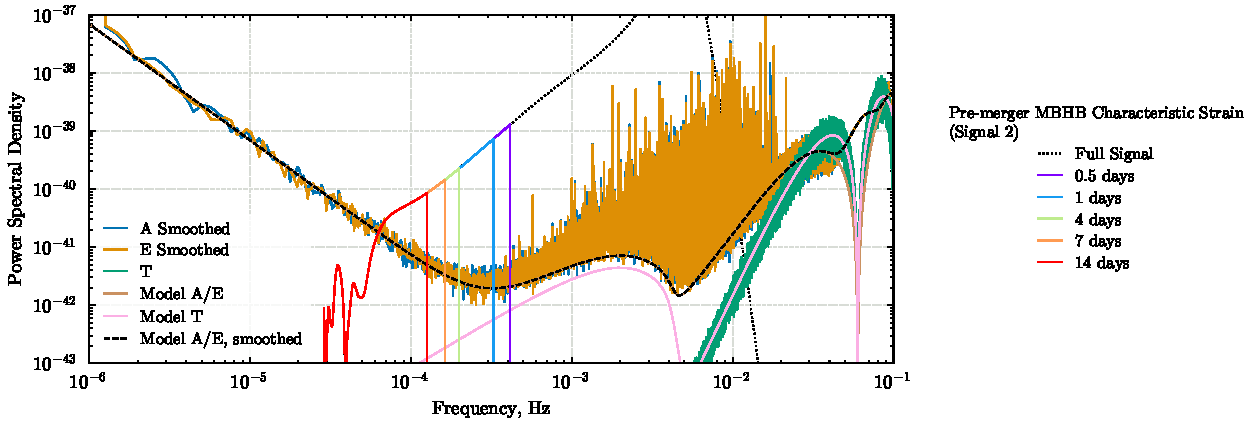
\includegraphics[width=\textwidth]{images/figure_X_psds_with_sources.pdf}
    \caption{
        Comparison of PSDs used in this work.
        The PSD is estimated from the Sangria dataset using the welch method with a segment duration of 18.25 days.
        The model shown is the noise model used to produce the Sangria dataset, and includes unresolvable galactic binary sources.
        Both the model and the estimated PSD require smoothing over the dip to zero at 0.06Hz.
        This smoothing is done using a Hann window to transition between the original PSD and a straight line between the peaks of the PSD model either side of the dip.
        We also show the characteristic strain for a MBHB signal from Sangria (Signal 4), which shows that at 14, 7 and 4 days-before-merger, the MBHB does not overlap
        the galactic binary confusion noise in frequency, but when the signal reaches around one day before merger,
        the galactic binary confusion noise starts to overlap with the signal.
    }
    \label{fig:psds}
\end{figure*}

\begin{table*}
    \begin{tabular}{|cc|c|ccccc|}
\hline
\multicolumn{2}{|c|}{Signal}& \multicolumn{6}{c|}{Expected SNR} \\
\hline
Number & Time  & Full Signal & 0.5 & 1 & 4 & 7 & 14 \\
\hline
0 & 55.56 & 2699.04 & 70.99 & 52.74 & 24.33 & 16.43 & 9.51 \\
1 & 101.23 & 105.72 & 3.99 & 2.49 & 0.79 & 0.47 & 0.28 \\
2 & 129.26 & 400.25 & 10.76 & 7.51 & 2.91 & 1.84 & 1.07 \\
3 & 130.31 & 1992.38 & 71.92 & 54.76 & 27.52 & 19.88 & 13.22 \\
4 & 133.41 & 3475.28 & 115.99 & 88.26 & 44.02 & 31.65 & 20.46 \\
5 & 138.55 & 427.13 & 16.40 & 10.79 & 3.85 & 2.37 & 1.22 \\
6 & 157.61 & 673.48 & 24.99 & 16.19 & 5.48 & 3.25 & 1.55 \\
7 & 191.34 & 579.12 & 15.72 & 10.70 & 4.02 & 2.56 & 1.49 \\
8 & 199.60 & 365.18 & 16.21 & 10.68 & 3.77 & 2.28 & 1.11 \\
9 & 215.34 & 392.96 & 18.69 & 12.41 & 4.75 & 3.12 & 1.82 \\
10 & 236.41 & 2187.78 & 45.09 & 31.90 & 12.71 & 8.13 & 4.37 \\
11 & 257.27 & 1200.55 & 45.32 & 33.31 & 13.99 & 8.92 & 4.71 \\
12 & 271.29 & 359.02 & 21.27 & 14.71 & 6.10 & 4.17 & 2.57 \\
13 & 282.51 & 823.00 & 24.75 & 18.00 & 7.81 & 5.23 & 3.00 \\
14 & 341.62 & 230.57 & 9.88 & 6.43 & 2.22 & 1.34 & 0.67 \\
\hline
\end{tabular}

    \caption{
        Characteristic SNRs for signals in the Sangria dataset.
        These are computed by comparing characteristic strain for the signal to the
        noise model PSD.
        We see that Signals 5 and 14 are unlikely to be seen even 0.5 days pre-merger, and 
        that signals 
    }
    \label{tab:characteristic_strain_snr}
\end{table*}

As a result, we can use the template banks from the zero-latency search paper without significant issues.

